\documentclass[a4paper,11pt]{article}
\pagestyle{headings}

\usepackage[utf8]{inputenc}
\usepackage[french]{babel}
\usepackage{graphicx}
\usepackage{float}
\usepackage{fullpage}
\usepackage{hyperref}
\usepackage{diagbox}
\usepackage{enumitem}
\usepackage[T1]{fontenc}
\graphicspath{{images/}}

\title{Reconnaissance de formes et apprentissage automatique Projet 1}
\author{Auriane Reverdell, Felix Hähnlein, Nicolas Violette, Romain Duléry}
\date{\today}

\setlength{\oddsidemargin}{0.2cm}
\setlength{\evensidemargin}{-0.7cm}
\setlength{\parindent}{30pt}
\setlength{\textwidth}{15cm}
\setlength{\textheight}{24cm}
\setlength{\topmargin}{-.5in}
\setlength{\parskip}{1ex}

\begin{document}

\maketitle
\vspace{1cm}

\section{Résumé du travail réalisé}

\section{Analyse des résultats expérimentaux}

    \subsection{Phase d'apprentissage}

	\subsubsection{Travail réalisé}

	\subsubsection{Analyse de l'influence des paramètres}

    \subsection{Détection faciale}

	\subsubsection{Détection de visage sans post-traitement}

	\subsubsection{Détection de visage avec post-traitement}

	\subsubsection{Évaluation des détections de visages}

\section{Conclusion}

\section{Notes Auriane pour qu'elle s'en rappelle}

    %TODO : faire une vraie analyse sur les paramètres

\section{Analyse qualitative des détections}
    
    \subsection{Orientation du visage}
	
	Dans l'image suivante (figure \ref{fig:visage_or1}), l'orientation du visage varie
	progressivement, cela nous montre exactement l'orientation à partir de laquelle la
	reconnaissance ne marche plus. Nous remarquons ici que la détection dépend de la présence
	des deux yeux, dès que l'un d'eux n'est plus visible ou occulté, la détection ne fonctionne
	plus.

	\begin{figure}[H]
	    \begin{center}
		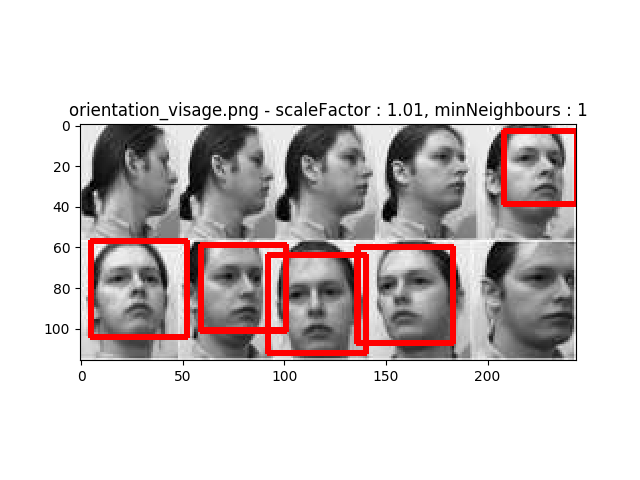
\includegraphics[scale = 0.6]{images/orientation_visage_1,01_1.png}
		\caption{Variation de l'orientation du visage - min neighbours = 1}
		\label{fig:visage_or1}
	    \end{center}
	\end{figure}

	Si l'on augmente \textit{minNeighbours}, rien ne change jusqu'à 3 (figure
	\ref{fig:visage_or2}) puis le nombre de TP diminue. En effet, cette variable
	(en l'augmentant) sert à limiter le nombre de FP. Or, comme il n'y a pas
	d'environnement d'arrière plan propices aux fausses détections, les fausses détections sont
	inexistantes, même avec un \textit{minNeighbours} à 1. Le \textit{scaleFactor} (à 1\%)
	permet,	quant à	lui, des détections précises (on ne saute pas trop rapidement à une petite 
	échelle).

	\begin{figure}[H]
	    \begin{center}
		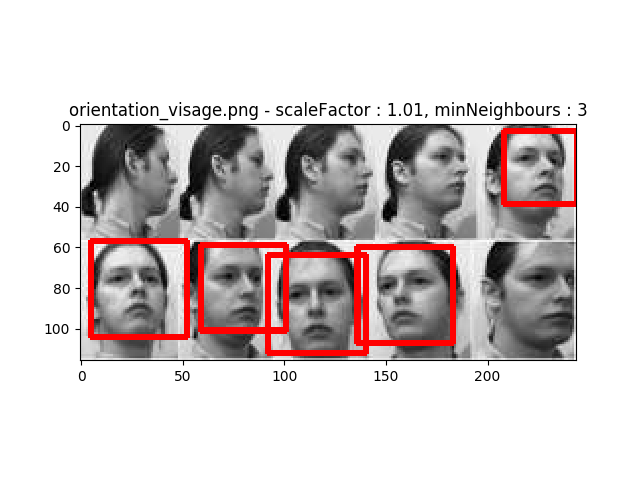
\includegraphics[scale = 0.6]{images/orientation_visage_1,01_3.png}
		\caption{Variation de l'orientation du visage - min neighbours = 3}
		\label{fig:visage_or2}
	    \end{center}
	\end{figure}

    \subsection{Expressions du visage}
	
	On pourrait se demander ce que deviennent les détections sur un visage avec des expressions
	différentes voire même avec les yeux fermés. On remarque sur la figure \ref{fig:visage_exp}
	que le détecteur est robuste à ces changements.

	\begin{figure}[H]
	    \begin{center}
		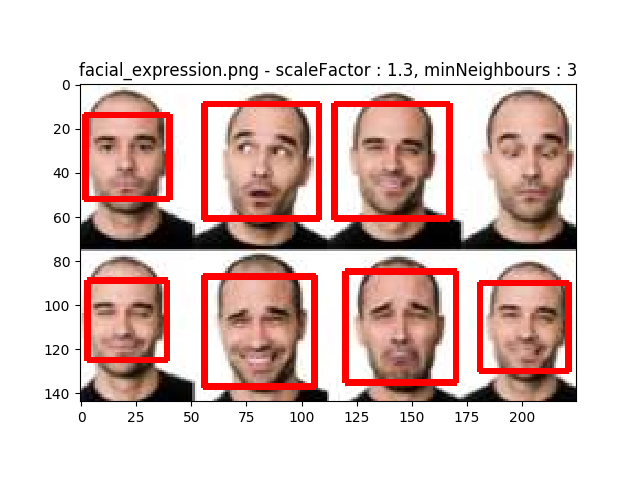
\includegraphics[scale = 0.6]{images/facial_expression_1,3_3.png}
		\caption{Changement d'expressions du visage}
		\label{fig:visage_exp}
	    \end{center}
	\end{figure}

    
    \subsection{Singes}

	Le singe est détecté lorsque le	\textit{scaleFactor} et le \textit{minNeighbours} sont
	relativement bas (figure \ref{fig:singe}), dès que l'on augmente à 1.06 le
	\textit{scaleFactor} la reconnaissance ne se fait plus correctement.
	En effet on peut supposer que les features sont moins
	adaptés aux variations de gris des visages des singes, i.e., même en mettant le
	\textit{minNeighbours} à 0 nous avons relativement peu de détections sur le vrai visage.

	\begin{figure}[H]
	    \begin{center}
		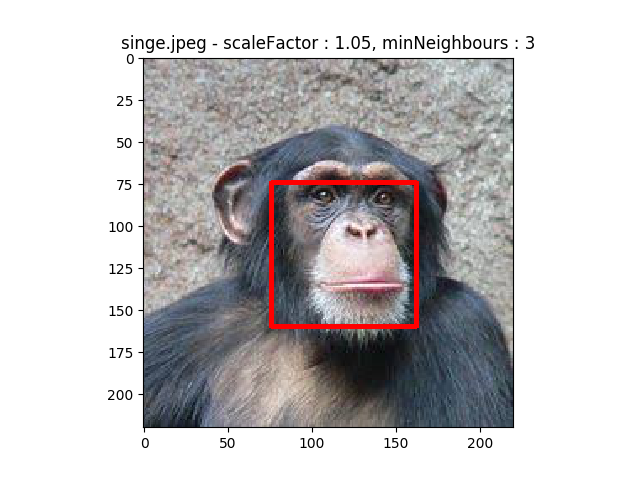
\includegraphics[scale = 0.6]{images/singe_1,05_3.png}
		\caption{Reconnaissance d'un singe}
		\label{fig:singe}
	    \end{center}
	\end{figure}

	Si l'on prend des paramètres identiques pour la reconnaissance du gorille (cela nous semble
	faisable car il y a une importante zone d'ombre au niveau des yeux du gorille), la
	reconnaissance ne marche pas, il faut augmenter le \textit{scaleFactor} à 1.02 pour qu'on
	ait une détection (cf figure \ref{fig:singe2}).

	\begin{figure}[H]
	    \begin{center}
		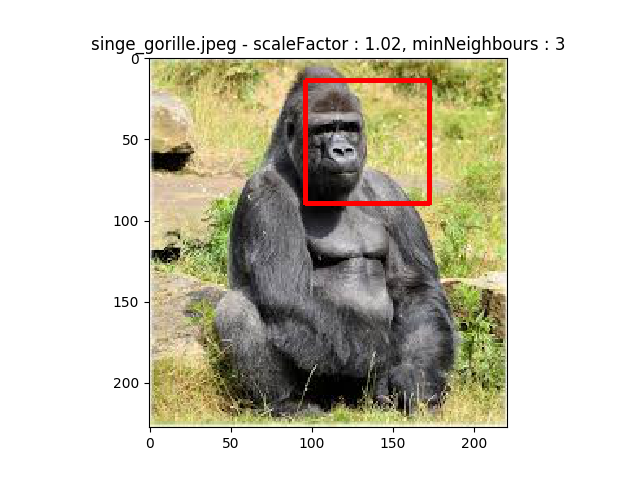
\includegraphics[scale = 0.6]{images/singe_gorille_1,02_3.png}
		\caption{Reconnaissance d'un gorille - scaleFactor = 1.02}
		\label{fig:singe2}
	    \end{center}
	\end{figure}

    \subsection{Occultations}
	
	Comme on l'a vu précédemment, lorsque qu'un oeil disparaît, la détection de visage ne se
	fait plus, on peut donc ce demander ce qui se passe dans le cas d'une occulation de la
	bouche ou encore dans le cas d'un déguisement de pirate.

	\subsubsection{Oeil de pirate}

	    Ce que l'on voit ici (figure \ref{fig:pirate}), c'est que, même si l'oeil est occulté, tant
	    que la partie des yeux est foncée, le visage est bien détecté alors que lorsque l'on
	    compare avec l'ocultation du visage par les mains (figure \ref{fig:mains}), il n'y a
	    plus de différentiel d'intensité (qui est ce sur quoi est basé l'algorithme de
	    Viola-Jones), les TP sont donc inexistants (même avec les paramètres au plus bas).

	    \begin{figure}[H]
	        \begin{center}
		   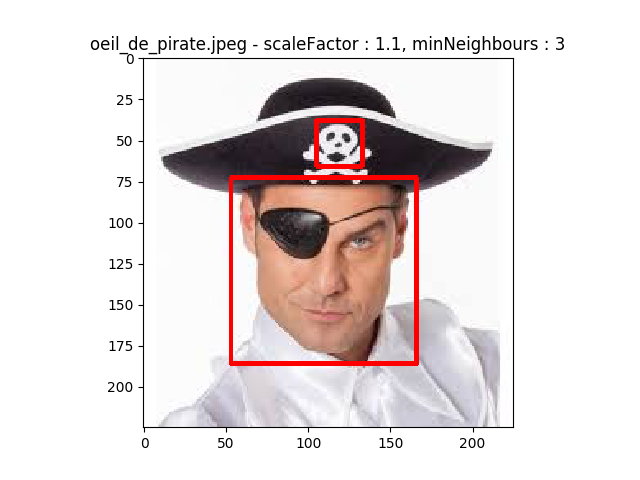
\includegraphics[scale = 0.6]{images/oeil_de_pirate_1,1_3.png}
		   \caption{Reconnaissance d'un visage occulté}
		   \label{fig:pirate}
	        \end{center}
	    \end{figure}

	    \begin{figure}[H]
	        \begin{center}
		   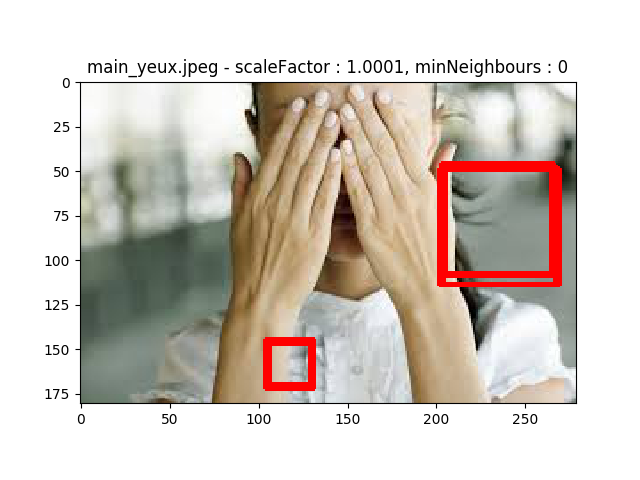
\includegraphics[scale = 0.6]{images/main_yeux_1,0001_0.png}
		   \caption{Reconnaissance d'un visage occulté par les mains}
		   \label{fig:mains}
	        \end{center}
	    \end{figure}

	\subsubsection{Lunettes de soleil}

	    Ces lunettes de soleil étant noires (figure \ref{fig:lunette}), la détection fonctionne très bien : il y a un gros
	    différentiel d'intensité entre les lunettes et le reste du visage.

	    \begin{figure}[H]
	        \begin{center}
		   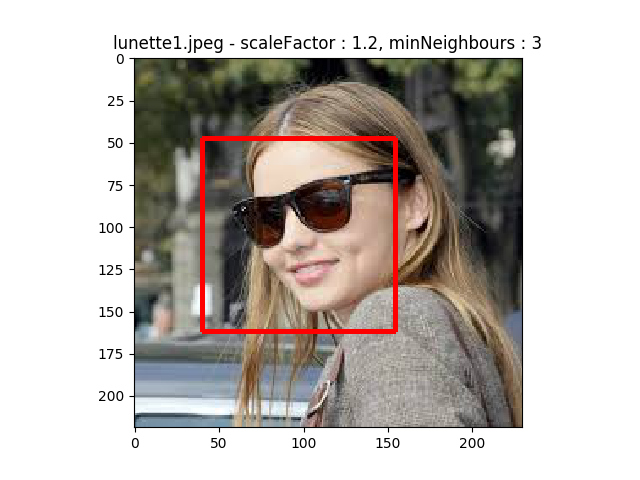
\includegraphics[scale = 0.6]{images/lunette1_1,2_3.png}
		   \caption{Reconnaissance d'un visage occulté par des lunettes de soleil}
		   \label{fig:lunette}
	        \end{center}
	    \end{figure}
	
	\subsubsection{Illumination}

	    Comme nous l'avons précisé, ci-dessus, la méthode de Viola-Jones est basée sur les
	    intensités. L'illumination est donc l'un des critères qui peut fortement affecter les
	    détections. En effet, un visage partiellement ombragé donnera du fil à retordre à
	    l'algorithme. \\

	    Lorsque l'on regarde la figure \ref{fig:illumination}, nous remarquons que les visages
	    non-détectés sont ceux qui ne laissent pas transparaître un \textit{feature} évident. Au
	    contraire, si l'on prend le visage en haut à droite, nous pouvons prédire qu'il
	    conviendra parfaitement à un \textit{feature} binaire.


	    \begin{figure}[H]
	        \begin{center}
		   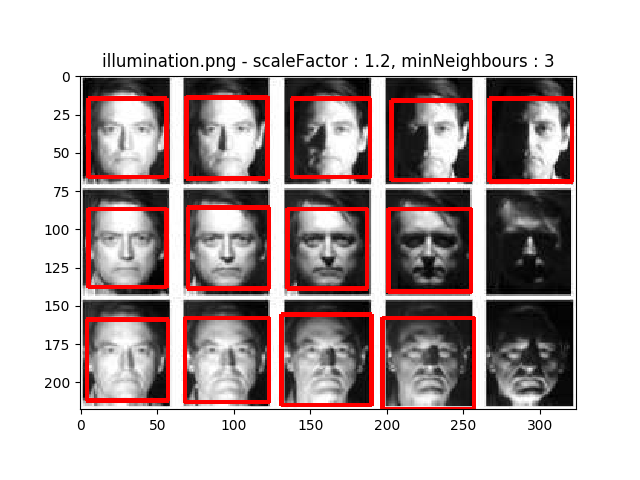
\includegraphics[scale = 0.6]{images/illumination_1,2_3.png}
		   \caption{Reconnaissance d'un visage ombragé}
		   \label{fig:illumination}
	        \end{center}
	    \end{figure}
	

\section{Bibliographie}

\hspace{-1.05cm}\url{http://www.ijcttjournal.org/2015/Volume25/number-1/IJCTT-V25P110.pdf} \\
\url{http://www-prima.inrialpes.fr/Prima/jlc/Courses/2017/PRML/Viola-Jones-CVPR2001.pdf} \\
\url{http://www.ipol.im/pub/art/2014/104/article.pdf}

\end{document}
